\documentclass[english]{article}
\usepackage{amsfonts}
\usepackage{tikz}
\usepackage{url}
\usepackage{graphicx,amsmath,amsthm,amssymb}
\usepackage{eucal}
\usepackage{color}
\usepackage[T1]{fontenc}
\usepackage{babel}
\usepackage{float}

\graphicspath{ {images/} }

\newcommand{\vect}[2]{\bigl[\begin{smallmatrix}#1\\#2\end{smallmatrix}\bigr]}
\newcommand{\vectt}[3]{\bigl[\begin{smallmatrix}#1\\#2\\#3\end{smallmatrix}\bigr]}
\newcommand{\Z}{\mathbb{Z}}
\newcommand{\R}{\mathbb{R}}
\newcommand{\C}{\mathbb{C}}
\newcommand{\CP}{\hat{\mathbb{C}}}

\title{A Space of Circle Packing Algorithms}

\author{
  Kevin Pratt\\
  \texttt{kevin.pratt@uconn.edu}
  \and
  Connor Riley\\
  \texttt{connor.riley@uconn.edu}
    \and
  Donald R. Sheehy\\
  \texttt{don.r.sheehy@uconn.edu}
}

\date{February 2016}
\begin{document}
\maketitle
\section{Introduction}
The Circle packing theorem was first discovered by Paul Koebe and then later reintroduced by William Thurston in 1985. As a result, this is a relatively new topic to many mathematicians and Computer Scientists. 
\section{Definitions}
The following section contains definitions needed either to explain other definitions or to understand Circle Packings to their fullest.
 \subsection{Graphs}
 
 A \textbf{graph} is an ordered pair $G=(V,E)$ which represents a set of objects where some of these objects are linked. In the denotation $G=(V,E)$, $V$ stands for the vertices or objects, and $E$ stands for the edges or links. Edges in a graph can be directed or undirected, however, we will focus on undirected edges in our application.

  A component or \textbf{connected component} of a graph is a subgraph in which any two vertices are connected to each other by a path which is connected to no additional vertices in the supergraph.

  A \textbf{loop} is when a vertex has an edge connecting it to itself.
  
  \begin{figure}[H]
  \centering
	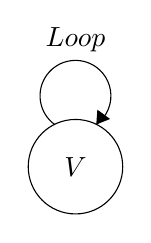
\begin{tikzpicture}[scale=0.2]\tikzstyle{every node}+=[inner sep=0pt]
	  \draw [black] (25.7,-24.2) circle (3);
	  \draw (25.7,-24.2) node {$V$};
      \draw [black] (24.377,-21.52) arc (234:-54:2.25);
      \draw (25.7,-16.95) node [above] {$Loop$};
      \fill [black] (27.02,-21.52) -- (27.9,-21.17) -- (27.09,-20.58);
    \end{tikzpicture}
    \caption{A loop.}
    \label{fig: loop}
  \end{figure}
  
  A graph with multiple edges is one which has two or more edges connect the same two vertices.\\
  
  \begin{figure}[H]
    \centering
	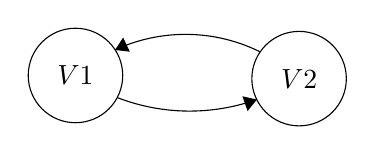
\begin{tikzpicture}[scale=0.2]\tikzstyle{every node}+=[inner sep=0pt]
	  \draw [black] (25.7,-24.2) circle (3);
	  \draw (25.7,-24.2) node {$V1$};
	  \draw [black] (39.9,-24.4) circle (3);
	  \draw (39.9,-24.4) node {$V2$};
	  \draw [black] (37.217,-25.726) arc (-70.44515:-111.16871:12.75);
	  \fill [black] (37.22,-25.73) -- (36.3,-25.52) -- (36.63,-26.46);
	  \draw [black] (28.21,-22.575) arc (114.84766:63.53848:10.656);
	  \fill [black] (28.21,-22.58) -- (29.15,-22.69) -- (28.73,-21.79);
	\end{tikzpicture}
	\caption{A graph with multiple edges.}
      \label{fig: multiple edges}
  \end{figure}

 \subsubsection{Types of Graphs}
  A graph is \textbf{connected} when there is a path between every pair of vertices. 
  In a connected graph every vertex is reachable. A graph with just one vertex is connected. A graph is said to be \textbf{k-connected} if there does not exist a set of k-1 vertices whose removal disconnects the graph. Typically we will work with 3-connected graphs - this means that three vertices would have to be removed to disconnect the graph.
  
  A \textbf{simple graph} is an unweighted, undirected graph, containing no loops or multiple edges. 
  A simple graph may either be connected or disconnected.
  
  A \textbf{planar graph} is one that can be embedded in the plane. 
  In other words, the graph can be drawn on the plane in such a way that its edges intersect only at their endpoints (no edges cross each other). By $Whitney's$ $Theorem$ if a graph is planar and 3-connected, all the faces of the graph will be the same shape. A Triangulated graph, or triangulation is an example of this property.
  
  A graph $G' = (V',E')$ is a \textbf{subgraph} of $G$ ($G' \subseteq G$), if $V' \subseteq V$ and $E' \subseteq E$. Two important types of subgraphs are:
  \begin{itemize}
  \item A $path$ between two vertices $v_1$ and $v_k$ in $G$ is a subgraph $G' \subseteq G$ with $V' = \{v_1,...v_k\}$ and $E' 	= \{\{v_1,v_2\},...\{v_{k-1}, v_k\}\}$. We write $G' = G_{v_1}^{v_k}$.
  \item A $k-cycle$ in $G$ is a subgraph $G'\subseteq G$ with $V' = \{v_1,...,v_k\}$ and $E' = \{\{v_1,v_2\},...\{v_{k-1}, v_k\}, \{v_k,_1\}\}$
  \item A $Y-Graph$ in $G$ that connects $v_1,v_2, v_3 \in V$ is a subgraph $G' \subseteq G$ such that there exists a vertex $w \in V \backslash \{v_1,v_2, v_3\}$ and paths $G_{v_1}^w, G_{v_2}^w, G_{v_3}^w$ that are disjoint except for the common endpoint $w$.
  \end{itemize}
  A \textbf{triangulation}, also referred to as a \textbf{maximal planar graph}, is a planar graph in which there is no way to add another edge and have the graph continue to be planar. In practice this means that each face is bounded by three edges
  
  \textbf{Euler's formula} states that if a finite, connected, planar graph is drawn in the plane without any edge intersections, and $v$ is the number of vertices, $e$ is the number of edges and $f$ is the number of faces (including the outer region), then: 
  \begin{equation} 
	v-e+f=2
  \end{equation}
  
  A \textbf{polytope} is a geometric object with flat sides that can exist in any number of dimensions. The $edge$ $graph$ $G(P)$ of a polytope $P$ is the graph whose vertex set is the vertex set of the polytope $P$. 
  
  \subsection{Embedding}
  A \textbf{simple arc} is an image of a continuous injective map [0,1] $\rightarrow \Sigma$.\\
  \begin{figure}[h]
      \centering
      \includegraphics[scale=.3]{simple_arcs}       
      \caption{Three simple arcs.}
      \label{fig: Figure 3}
  \end{figure}\\
  An \textbf{embedding} of a graph $G$ on a surface $\Sigma$ is a representation of $G$ on $\Sigma$ in which points of $\Sigma$ are associated to vertices and simple arcs are associated to edges in such a way that:
  \begin{itemize}
	\item The endpoints of the arc associated to the edge $e$ are the points associated to the end vertices of $e$.
	\item No arcs include points associated with other vertices.
	\item Two arcs never intersect at a point which is interior to either of the arcs.
  \end{itemize}
  This can be stated mathematically as the following: Given edges $e=(u,v)$, the function mapping the vertices to the plane $ \phi :V \rightarrow \R^2$, and the function mapping the edges to the plane $ \rho_e :[0,1] \rightarrow \R^2$, the embedding $= <\phi, \{\rho_e\} \in E >$
  \subsubsection{Straight-Line Embedding}
  A \textbf{straight-line embedding} is a embedding of a planar graph in which all arcs are straight.


  If $c$ is the number of components in a graph, then a more general form of Euler's formula is:
  \begin{equation} 
	v-e+f= 1 + c
  \end{equation}
  
  \subsubsection{Delaunay Triangulation}
  The \textbf{circumcircle} of a triangle is the circle which passes through all three of its vertices. The center of the circumcircle is called the \textbf{circumcenter} and the radius is the \textbf{circumradius}. The circumcenter can be found by finding the intersection of the \textbf{altitudes}, which are formed by drawing a perpendicular line from each vertex to the opposite side of the triangle. The \textbf{orthocircle} is the circle that is orthogonal to the disks around the vertices of a triangle. These disks determine the weight of each vertex of the triangle. If these disks have radii equal to zero, then the orthocircle is equal to the circumcircle.
  
  A \textbf{Delaunay Triangulation} for a set of points $P$ is the triangulation of those points such that no point in $P$ is inside the circumcircle of any other triangle. These triangulations are intimately connected to Circle Packings, described later.
  
  The \textbf{Voronoi Diagram} is the dual of the Delaunay Triangulation. If you input $n$ points in $\R^2$ $P=\{p_1,..p_n\}$ the output is a polyhedral complex with $n$ 2-face (2-cells) where cell $v_i$ is $v_i = \{x \in \R^2 : \| x - p_i \| \leq \| x - p_j\|\}$
 
 \subsection{Tutte Embedding}
   Given a graph $G=(V,E)$ to each edge $\{i,j\}\in\sigma$ we assign as weight $w_ij\in\R$ also known as a \textbf{stress} that represents the elasticity constant of the corresponding rubber band. $w_ij$ must be equivalent to $w_ji$. A negative weight means that the ege is pushing on its two endpoints, whereas a positive weight means that the edge is pulling on the endpoints. 
 A \textbf{lifting} (of a planar straight line graph) is an assignment of heights to vertices such that the vertices of each face are coplanar in $\R^3$ (the faces are flat).
  
  A \textbf{Tutte embedding} or barycentric embedding of a simple 3-connected planar graph is a crossing-free straight-line embedding with the properties that the outer face is a convex polygon and that each interior vertex is at the average (or barycenter) of its neighbor's positions. If the outer polygon is fixed, this condition on the interior vertices determines their position uniquely as the solution to a system of linear equations. Solving the equations geometrically produces a planar embedding. 
  
  Tutte's spring theorem states that this unique solution is always crossing-free, and more strongly that every face of the resulting planar embedding is convex. It is called the spring theorem because such an embedding can be found as the equilibrium position for a system of springs representing the edges of the graph.
  
  Algorithm: First, fix one face of a simple, planar, 3-connected graph in convex position. Next, place each other vertex at the barycenter(centroid) of its neighbors. The result is a non-crossing, convex drawing.
 
 Tutte's Theorem: Let $G = (\{1,...,n\},E)$ be a 3-connected planar graph that has a face $(1,...,k)$ for some $k<n$. Let $p_1,...,p_k$ be the vertices of a convex k-gon. Let $E'$ be the set of interior edges and let $w : E \rightarrow \R^+$ be an assignment of positive weights to the interior edges. Then,
 	\begin{itemize}
		\item There are unique equilibrium positions $p_{k+1}, ...p_n \in \R^2$ for the interior vertices. 
		\item All faces of $G$ are realized as non-overlapping convex polygons.
	\end{itemize}
	
	
\subsubsection{Proof of Tutte's Theorem}
Let $\omega : E \rightarrow \R$ be an assignment of weights to the edges of a graph and let $p:V \rightarrow \R^2$ be an assignment of positions in $\R^2$ for the vertices of $G$. A vertex $v \in V$ is in equilibrium if  $\sum\limits_{\{v,w\} \in E} \omega_{v,w}(p_v - p_w) = 0$

\textsc {Proof of Existence and Uniqueness}  Assume that the positions of the peripheral points $p_v = (x_v,y_v); v \in \{k+1,...,n\}$ are given. We have to prove that suitable positions $p_v = (x_v,y_v); v \in \{1,...,k\}$ for the interior vertices exist and that these positions are unique. Without loss of generality we may assume that $p_n = (0,0)$. Consider the function
\begin{center}
$E(x_1,...,x_k,y_1,...,y_k) = \frac{1}{2} \sum\limits_{\{v,w\} \in E'} \omega_{v,w}((x_v - x_w)^2 + (y_v - y_w)^2) 
= \frac{1}{2} \sum\limits_{\{v,w\} \in E'} \omega_{v,w} \|p_v - p_w\|^2$. \\
\end{center}
$E$ is a quadratic function that is non-negative everywhere. Assume that $z=(x_1,...x_k,y_1,...y_k)$ has at least one entry (say $x_i$) with large absolute value. This implies that $p_i$ is far away from the point $p_n = (0,0)$. Since $G$ is connected, there is a path that connects $p_i$ with $p_n$ and for at least one edge $(v,w)$ in this path the distance $\|p_v - p_w\|$ is large. Since the squared distances are weighted with positive coefficients $E(z)$ is also large. Thus for sufficiently large $\alpha > 0, \|z\| > \alpha$ implies $E(z) > E(0)$. This means that $E$ must be strictly convex and thus takes its unique minimum on $\{z | |z| < \alpha \}$. The assertion follows from the observation that the condition for a critical point $(\triangledown E = 0)$ of $E$ is
\begin{center}
$\frac{\delta E}{\delta x_i} = \sum\limits_{\{v,w\} \in E'} \omega_{v,w}(x_v - x_w) = 0$ and $\frac{\delta E}{\delta x_i} = \sum\limits_{\{v,w\} \in E'} \omega_{v,w}(y_v - y_w) = 0$
\end{center}
for all $i \in \{1,..,k\}$. This is exactly the equilibrium condition for the interior vertices.

Another variant of Tutte's theorem for non-strictly convex boundaries is as follows:

 \subsection{Maxwell-Cremona Theorem}
 Theorem: (1) Let $G[p]$ be a planar framework with a convex outer face $F$. There is a correspondence between
 \begin{itemize}
 	\item positive stresses on the interior edges which are in equilibrium at all interior vertices
	\item concave piecewise linear liftings of $G$.
 \end{itemize}
 (2) Let $G[p]$ be a planar framework with a convex outer face $F$. There is a correspondence between
 \begin{itemize}
 	\item stresses which are positive on all interior edges and negative on all boundary edges and which are in equilibrium at all vertices,
	\item concave piecewise linear liftings of $G$ such that the boundary edges are horizontal,
	\item convex polytopes $P$ projecting on $G$
 \end{itemize}
 (3) Let $G[p]$ be the union of two planar frameworks which share a common convex outer face $F$. There is a correspondence between:
 \begin{itemize}
 	\item stresses which are positive on all interior edges and negative on all boundary edges and which are in equilibrium at all vertices.
	\item convex polytopes $P$ projecting on $G$.
 \end{itemize}
 
 The boundary of $F$ corresponds to the edges and vertices which vertical supporting planes, and the two planar frameworks correspond to the upper half and the lower half of $P$.
 
 The \textbf{Maxwell-Cremona Theorem}: There is a natural correspondence between equilibrium stresses of planar linkage and the liftings of that linkage. 
 
 $Equalibruim$  $Stress \leftrightarrow Reciprocal$ $Diagrams \leftrightarrow Liftings$
 
\subsubsection{Proof of the Maxwell-Cremona Theorem}
An \textbf{edge patch} is written as $<h,i;j,k>$. We say it joins the vertices $h,i$ and separates the faces $j,k$.
\begin{figure}[h]
      \centering
      \includegraphics[scale=.3]{edge_patch}       
      \caption{The edge patch $<h,i;j,k>$.}
      \label{fig: Figure 4}
  \end{figure}\\
  
A \textbf{framework} in the plane is a finite graph $G=(V,E)$ and a mapping $p: V \rightarrow \R^2$ such that $p(a) \neq p(b)$ if $(a,b) \in E$. The notation for frameworks is as follows: 

\begin{itemize}
	\item The framework is written as $G(p)$
	\item $p(a)$ is a point treated as a position vector. 
	\item Joints are written as $p(i)$ or more commonly $p_i$.
	\item Bars are written as $p_ip_j$ or $\{i,j\}$
	\item Edges are written $ij$.
\end{itemize}

The forces exerted by a bar are a pair of forces along the bar equal in magnitude but opposite in direction. $\omega_{ij}(p_j - p_i)$ at $p_i$ and $\omega_{ij}(p_i - p_j)$ at $p_j$. If $\omega_{ij} \geq 0$ the force is a tension force, otherwise it is a compression force. The forces at a joint $p_i$ are at equilibrium if $\sum_j \omega_{ij}(p_j-p_i) = 0$.

A \textbf{cut} is a partition of the vertices of a graph into two disjoints subsets.

An \textbf{annulus} is a ring-shaped object bounded by two concentric circles. 

A \textbf{self stress} on a framework $G(p)$ is an assignment of scalars $\omega_{ij}$ to the edges such that for each vertex $i : \sum_j \omega_{ij}(p_i - p_j) = 0$. 
\begin{itemize}
	\item A self stress is non-trivial if some $\omega_{ij} \neq 0$.
	\item A self stress is full if all $\omega_{ij} \neq 0$.
	\item A framework is independent if it supports only the trivial self stress with all scalars zero.
	\item The support is the set of edges on which $\omega_{ij} \neq 0$.
	\item The self stress is full if the support is the entire graph.
\end{itemize}
A \textbf{combinatorial oriented polyhedron} is a finite set of vertices, faces and edge patches such that:
\begin{enumerate}
	\item if $<h,i;j,k> \in E$ then $<i,h;k,j> \in E$ but $<h,i;k,j> \not\in E$ and $<h,i;j,k> \not\in E$.
	\item For each vertex $a_0$ all edge patches with first entry $a_0$ form a cycle $<0,i_s;j_s,k_s>$ for $1\leq s \leq t$ $t\geq3$ with $k_s = j_s + 1$ and $j_t = k_1$ where all $k_s$ and $i_s$ are distinct. 
	\item For each face $F^0$ all edge patches with last entry $F^0$ form a cycle $<h_s, i_s;j_s,0>$ for $1\leq s \leq t$ $t\geq3$ with $i_s = h_s + 1$ and $i_t = h_1$ where all $h_s$ and $j_s$ are distinct.
	\item Each pair $a_0$, $a_1$ is joined by a vertex edge path. Each pair of faces is connected by a face-edge path. 
\end{enumerate}

\subsubsection{Spherical Combinatorial Polyhedron}
A combinatorial polyhedron is spherical if every closed path of faces and distinct edges $<h_r,i_r;j_r,k_r>$ for $1 \leq r \leq t$ such that $j_{r+1} = k_r$ and $j_1 = k_t$ disconnects the vertices. If so, then the dual is also spherical. 

A graph $G$ is a graph of a spherical combinatorial polyhedron if and only if its is vertex 2-connected and edge 3-connected. Ie. the graph of a spherical polyhedron is planar.

\textsc{Proof}
Part A: First we must show that the graph is vertex 2-connected and edge 3-connected. We already know the graph is connected from property 2 above. We prove this by contradiction. First we assume the graph an be separated by removing $v_0$. Next we select $C$ surrounded by an annulus in the sphere, reinserting $v_0$. We must insert wedges from $C$ to $v_0$, around $C$ this breaks the annulus into a single face contacting $v_0$ twice. This contradicts property 3 from above.
To show the graph is edge 3-connected we assume that removing 2 edges disconnects the graph and prove by contradiction. These two edges go from $\{a,a^{'}\}$ and $\{b, b^{'}\}$ joining 2 components. The two edges cut out two faces $F^1$ and $F^2$. In the cycle around $F^1$, the face $F^2$ now occurs across two edges. This contradicts property 3 of the combinatorial oriented polyhedron.

Part B:
Given any vertex 2-connected, edge 3-connected graph, we form a corresponding combinatorial spherical polyhedron: arcs and vertices surround simple disks which become faces along with the outer face. After placing point $f^j$ in each face we add $<h,i;j,k>$ if and only if the circuit $p_h, f^i,p_i,f^k$ around an arc $d_{ij}$ is clockwise. 

\begin{enumerate}
	\item Clearly the patches are each vertex form a cycle. Since we do not have a multi-graph the vertices are distinct. If a cycle around a vertex contained a face twice, then the graph could be disconnected by removing this vertex. This contradicts the vertex 2-connectivity. 
	\item Clearly the patches around a face form a cycle. Assume a vertex occurs twice in a cycle. Since there are no loops removing it violates 2-connectivity. Assume an adjacent face in a cycle occurs twice, removing edges violates 3-connectivity.
\end{enumerate}

\subsubsection{Proof of Maxwell Cremona Theorem}
A reciprocal framework $H* = ((F,E);P)$ on the dual combinatorial polyhedron is a framework such that for each edge patch $<h,i;j,k>$  the vector $v_e = p_i - p_h$ is perpendicular to the vector $v^e = p^k - p^j$ from the reciprocal. \\
\\
\textsc{Theorem} A plane framework on a planar vertex 2-connected, edge 3-connected graph, supports a self stress if and only if it has a reciprocal framework. \\
\\
\textsc{Proof} Starting with a planar drawing of a graph, form the associated spherical polyhedron. 

A note on notation: $90^o$ clockwise rotation will be written $u^\bot$ and $90^o$ counter-clockwise rotation will be written $-u^\bot$

Part A: Assume the spherical polyhedron has a reciprocal framework.
For each edge patch $<h,i;j,k>$ we will use the equation $\omega_{hi}(p_i - p_h) = -(P^k - P^j)^\bot$ or $\omega_ev_e = (V^e)^\bot$ to define scalars $\omega_{hi} = \omega_e$. All scalars will not equal zero because $P^j \neq P^k$ in a framework. From the facial polyhedrons of the reciprocal framework we get $\sum\omega_ev_e = 0 = \sum\omega_{hi}(p_i - p_h)$

Part B: Assume we have a full self stress on the framework.
Pick a face $F^0$ and a point $P^0$ for the this face. Any other face is connected by a simple face-edge path of edge patches $\{...e...\}$. We define $P^1 = P^0 + \sum\omega_ev_e^\bot$. This is a consistent definition provided that two different paths from $F^0$ to $F^1$ give the same point $P^1$. Two such paths form a closed path on the spherical polyhedron and therefore the edges of the path form a cut set for the graph of the polyhedron. If we travel on one path and back on the other we see the sums on the two paths are equal, as required $\sum\omega_ev_e = \sum\omega_e^{'}v_e^{'} = 0$ For each edge $e = <i,h;j,k>$ the path from $P^j$ to $P^k$ is this single edge and the difference in position is $P^j - P^k = -\omega_ev_e^\bot$. Thus, we have a true reciprocal.

These results generalize to any combinatorial oriented polyhedron. \\
\\
\textsc{Theorem} Given a combinatorial oriented polyhedron $(V,F,E)$ and any framework $H = ((V,E);P)$ there is a full self stress on the framework satisfying $\sum \omega_ev_e = 0$ if and only if there is a reciprocal framework $H* = ((F,E);P)$. 

\textsc{Proof} Part A: Given a reciprocal there is a full self stress.
For any face-edge cycle $\omega_e v_e = (V^e)^{\bot}$ since the vectors $V^e$ form a closed polygon in the reciprocal $\sum_e(V^e)^\bot = 0$.

Part B: Given a full self-stress $P^1 = P^0 + \sum_e \omega_ev_e^\bot = reciprocal$
Given any two paths between $F^0$ and $F^1$ we get the same value for $P^1$ since the sum up one path and back the other is a cycle and yields zero.


 
  \subsection{Topology}
 Topology is concerned with the properties of space that are preserved under continuous deformations, such as stretching and bending, but not tearing or gluing. This can be studied by considering a collection of subsets, called open sets, that satisfy certain properties, turning the given set into what is known as a topological space. 
  \subsubsection{Riemann Surface}
  To understand Riemann surfaces, one must first understand the complex plane. The complex plane is a geometric representation of the complex numbers, where the x-axis represents the real part of a complex number and the y-axis the complex part. Riemann surfaces may be thought of as deformed versions of the complex plane. These surfaces are important for studying Holomorphic functions, also called conformal maps, which are complex-valued functions of one or more complex variables that is complex differentiable in a neighborhood of every point in its domain.
  
  The most important Riemann surface for Circle Packing is the Riemann Sphere which is a model of the complex plane plus a point at infinity. The Riemann sphere can be visualized as the unit sphere in $\mathbb{R}^3$. 


 \subsection{Circle Packing}
  We say that two circles drawn in a plane kiss (or osculate) when they intersect in exactly one point. 
  A \textbf{circle packing} is a graph formed by a set of circles which have no overlapping interiors, where each circle kisses its surrounding circles.
  
  Formally, a collection $P = \{c_v\} $ of circles in $G$ is said to be a circle packing for a complex $K$ if $P$ has a circle $c_v$ associated with each vertex $v$ of $K$, two circles $c_u$ and $c_v$ are (externally) tangent whenever $<u,v>$ is an edge of $K$, and three circles $c_u$, $c_v$, $c_w$ form positively oriented triple in $G$ whenever $<u,v,w>$. forms a positively oriented face of $K$.
   
  The \textbf{intersection graph} of a circle packing is the graph having a vertex for each circle and an edge for every pair of circles that are tangent. 
  If the circle packing is on the plane or the sphere, then its intersection graph is called a \textbf{coin graph}. 
  Coin graphs are always connected, simple and planar. 

    Common geometric settings for circle packing are the $euclidean$ $plane$, $the$ $sphere$ and the $hyperbolic$ $plane$. Each pair of circles in a packing forms a tangent pair, and the empty space between each $triple$ forms a $interstice$. A $flower$ is the next level of structure, which consists of a central circle and some number of $petal$ circles. The number of petals defines the $degree$ of the central circle. A condition that we will enforce on all circle packings is that every circle must have a flower. This condition is a $local$ $planarity$ condition. Note that while not all circle packings are unilevant, the ones created by our application will all be unilevant. This means that the interior of all the circles will be mutually disjoint and that the angle sum at each label will be $2\pi$.
    
    Every circle packing is also a Weighted Delaunay triangulation. In the triangulation the weighted disks assigned to the vertices to find the orthocenter end up being the circles in the packing and the orthocircle becomes the inscribed circle of the triangle. 
    
    \subsubsection{Koebe Representation Theorem}
    Given any planar graph $G$ with vertex set $V(G) = \{v_1, ... v_n \}$ and edge set $E(G)$, we can find a packing of n (not necessarily congruent) circular discs $C= \{C_1,... C_n\}$ in the plane with the property that $C_i$ and $C_j$ touch each other if and only if $v_i v_j \epsilon E(G)$ for $1 \le i \le n$.
    \subsubsection{Stereographic Projections}
    A \textbf{sterographic projection} is a bijective mapping that projects a sphere onto a plane.
     The projection is defined on the entire sphere except for the projection point. 
    As the mapping is bijective there exists an inverse mapping from the plane to the sphere.

    \subsubsection{Mobius Transformations}
    A \textbf{M\"{o}bius Transformation} of a plane can be obtained by performing the stereographic projection of the plane onto a sphere, then rotating or moving the sphere and then performing the sterographic projection back onto the plane. 
    Formally, a M\"{o}bius Transformation is a rational function defined on the extended complex plane $\CP = \C\cup\{\infty\}$ of the form:
    \begin{equation} 
    	f(z) = \frac{az+b}{cz+d}
    \end{equation}
    where $z\in\CP$ is a complex variable and $a,b,c,d\in\CP$ are complex numbers such that $ad - bc$ $\neq$ $0$.
 
 \subsection{Dual}
  The dual of a point is a line. The mapping is as follows: $p : point = \vect{p_x}{p_y} \rightarrow p^* : line = \vect{2p_x}{-p_y}$ The mapping from a line to a point is: $\ell : line = \vect{\ell_n}{\ell_b} \rightarrow \ell^* : point = \vect{\frac{1}{2}\ell_n}{-\ell_b}$.
  
  The \textbf{dual graph} of a plane graph $G$ is a graph that has a vertex for each face of $G$. 
  The dual graph has an edge whenever two faces of $G$ are separated from each other by an edge. 
  Thus each edge $e$ of $G$ has a corresponding dual edge, the edge that connects the two faces on either side of $e$. 

  \subsubsection{Dual Packing}
  The \textbf{dual packing} is the circle packing of the dual graph. 
  In this packing, each circle passes through the points where the original circles kiss. 
  The dual packing does not form a triangulation whereas the original circle packing does.
  The dual radii are the radii of the circles in the dual packing, the dual stress and dual lifting are calculated similarly.

\section{Data Structure}
 \subsection{Half Edge}
  Also called a doubly-connected edge list, the \textbf{half edge} data structure associates two directed half edges to each edge on the graph. 
  Each half edge stores a vertex, a face, the next half edge, the previous half edge and the twin, which is the half edge going in the other direction. 
  Half edges are typically directed counter clockwise with respect to the face they define.
\subsection{Graph Structure}
  Let $G=(V,E)$ be a simple, planar, 3-connected graph. This graph will be composed of: $E$ edges, each bi-directional and made up of 2 Half Edge; $V$ vertices; and $F$ faces where a face is defined as $f(u,v) =$ face left of $\overrightarrow{uv}$ if $(u,v)\in E$.
\subsection{Enriched Embedding}
  In addition to storing the graph, we store other objects to allow for easier computation and to facilitate the switching of visual representations of the packing. These objects include the Embedding $\pi : V \rightarrow \mathbb{R}^2$, the Dual Embedding $\overline{\pi} : F \rightarrow \mathbb{R}^2$, the Stress $S : E \rightarrow \mathbb{R}$, the Lift $h : V \rightarrow \mathbb{R}$, the radii $r : V \rightarrow \mathbb{R}$ and the Dual Radii $\overline{r} : F \rightarrow \mathbb{R}$.

\section{Steinitz's Theorem}
 A graph $G$ is the edge graph of a 3-polytope if and only if $G$ is simple, planar and 3-connected.
 
 To prove this theorem, we must prove it in both directions. This proof will rely on the following facts:
 Let $G$ be a graph.
 \begin{enumerate}
 	\item (Menger's Theorem) If $G$ is 3-connected, then between any pair of vertices there are three paths $G_1, G_2, G_3$ in $G$ that are disjoint except for the endpoints.
	\item If there are three vertices $u,v,w$ that are connected by three different Y-graphs $Y_1, Y_2, Y_3$ that are disjoint except for $u,v,w,$ then $G$ is not planar.
	\item (Whitney's Theorem) If G is planar and 3-connected then the set $cells(G,D)$ is independent on the particular choice of drawing $D$ of $G$.
	\item (Euler's Theorem) If $G$ is planar and 2-connected and $D$ is a drawing of $G$ then the numbers of cells $c= \|cells(G,D)\|$, vertices $v = \|V\|,$ and edges $e = \|E\|$ are related by  $v+c = e+2$.
	
 \end{enumerate}

\section{Computing Delaunay Triangulations}
\subsection{Naive Algorithm}
If a triangle is not locally Delaunay, one of its edges can be flipped to create a locally Delaunay triangle. Therefore, a simple algorithm is to create a triangulation and flip the edges until all triangles are Delaunay. If $n$ is the number of edges, this algorithm can take $O(n^2)$ in the worst case and also does not work in three dimensions or higher.
\subsection{Incremental}
This algorithm  functions by repeatedly adding one vertex at a time and retriangulating the affected parts of the graph. When a vertex $v$ is added, the triangle containing $v$ is split into three and then the flip algorithm is applied. It takes $O(n)$ time to find the triangle containing $v$ and $O(n^2)$ time to run the flip algorithm. Therefore the total runtime is the same as the naive approach, $O(n^2)$. However, the incremental algorithm does have some advantages over the naive approach. First, if the vertices are inserted in a random order, on average only $O(1)$ triangles will be flipped. Finding the triangle containing $v$ can also be improved by storing the history of the splits and flips performed. Each triangle can store a pointer to a triangle that contains $v$ until we find a triangle that has not yet been replaced. On average this will take $O(log(n))$, therefore, for all vertices it takes $O(nlog(n))$. Lastly, this technique does extend beyond 2 dimensions, but the runtime can be exponential in the dimension. 
\subsection{Divide and Conquer}
This algorithm computes the Triangulation by recursively drawing a line to split the vertices into two sets. The triangulation is computed for each set and then the two sets are merged along the splitting line. The merge operation can be done in $O(n)$ time, so the total time is $O(nlog(n))$.

\section{Computing Circle Packings}
Given a planar, triangulated graph, begin with a set of tentative radii that do not correspond to a valid packing. Next, choose a internal vertex $v$ and calculate the total angle $\theta$ that its $k$ neighboring circles would cover around the circle for $v$, if the neighbors were placed tangent to each other and to the central circle using their tentative radii. Next, determine a representative radius $r$ for the neighboring circles, such that $k$ circles of radius $r$ would give the same covering angle $\theta$ as the neighbors of $v$ give. Lastly, set the new radius for $v$ to be the value for which $k$ circles of radius $r$ would give a covering angle of exactly $2\pi$.


\bibliographystyle{plain}
\bibliography{references}
\end{document}















